% !TEX TS-program = XeLaTeX
% use the following command:
% all document files must be coded in UTF-8
\documentclass[portuguese]{textolivre}
% build HTML with: make4ht -e build.lua -c textolivre.cfg -x -u article "fn-in,svg,pic-align"

\journalname{Texto Livre}
\thevolume{19}
%\thenumber{1} % old template
\theyear{2026}
\receiveddate{\DTMdisplaydate{2025}{7}{18}{-1}} % YYYY MM DD
\accepteddate{\DTMdisplaydate{2026}{3}{18}{-1}}
\publisheddate{\DTMdisplaydate{2026}{4}{18}{-1}}
\corrauthor{Eusebio Fernando Chitlango}
\articledoi{10.1590/1983-3652.2026.60397}
%\articleid{NNNN} % if the article ID is not the last 5 numbers of its DOI, provide it using \articleid{} commmand 
% list of available sesscions in the journal: articles, dossier, reports, essays, reviews, interviews, editorial
\articlesessionname{articles}
\runningauthor{Chitlango} 
%\editorname{Leonardo Araújo} % old template
\sectioneditorname{Fernando da Costa Barbosa~\orcid{0000-0001-8558-3521}}
\layouteditorname{Saula Cecília~\orcid{0009-0006-3069-8480}}

\title{Uso do vídeo na aprendizagem: uma experiência na projeção diédrica de ponto}
\othertitle{Use of video in learning: an experience in point dihedral projection}
% if there is a third language title, add here:
%\othertitle{Artikelvorlage zur Einreichung beim Texto Livre Journal}

\author[1]{Eusébio Fernando Chitlango~\orcid{0009-0000-9574-0797}\thanks{Email: \href{mailto:chitlangodesenho@gmail.com}{chitlangodesenho@gmail.com}}}
\affil[1]{Universidade Federal de Minas Gerais, Escola de Arquitetura e Design, Belo Horizonte, MG, Brasil.}

\addbibresource{article.bib}
% use biber instead of bibtex
% $ biber article

% used to create dummy text for the template file
\definecolor{dark-gray}{gray}{0.35} % color used to display dummy texts
\usepackage{lipsum}
\SetLipsumParListSurrounders{\colorlet{oldcolor}{.}\color{dark-gray}}{\color{oldcolor}}

% used here only to provide the XeLaTeX and BibTeX logos
\usepackage{hologo}

% if you use multirows in a table, include the multirow package
\usepackage{multirow}

% provides sidewaysfigure environment
\usepackage{rotating}

% CUSTOM EPIGRAPH - BEGIN 
%%% https://tex.stackexchange.com/questions/193178/specific-epigraph-style
\usepackage{epigraph}
\renewcommand\textflush{flushright}
\makeatletter
\newlength\epitextskip
\pretocmd{\@epitext}{\em}{}{}
\apptocmd{\@epitext}{\em}{}{}
\patchcmd{\epigraph}{\@epitext{#1}\\}{\@epitext{#1}\\[\epitextskip]}{}{}
\makeatother
\setlength\epigraphrule{0pt}
\setlength\epitextskip{0.5ex}
\setlength\epigraphwidth{.7\textwidth}
% CUSTOM EPIGRAPH - END

% to use IPA symbols in unicode add
%\usepackage{fontspec}
%\newfontfamily\ipafont{CMU Serif}
%\newcommand{\ipa}[1]{{\ipafont #1}}
% and in the text you may use the \ipa{...} command passing the symbols in unicode

% LANGUAGE - BEGIN
% ARABIC
% for languages that use special fonts, you must provide the typeface that will be used
% \setotherlanguage{arabic}
% \newfontfamily\arabicfont[Script=Arabic]{Amiri}
% \newfontfamily\arabicfontsf[Script=Arabic]{Amiri}
% \newfontfamily\arabicfonttt[Script=Arabic]{Amiri}
%
% in the article, to add arabic text use: \textlang{arabic}{ ... }
%
% RUSSIAN
% for russian text we also need to define fonts with support for Cyrillic script
% \usepackage{fontspec}
% \setotherlanguage{russian}
% \newfontfamily\cyrillicfont{Times New Roman}
% \newfontfamily\cyrillicfontsf{Times New Roman}[Script=Cyrillic]
% \newfontfamily\cyrillicfonttt{Times New Roman}[Script=Cyrillic]
%
% in the text use \begin{russian} ... \end{russian}
% LANGUAGE - END

% EMOJIS - BEGIN
% to use emoticons in your manuscript
% https://stackoverflow.com/questions/190145/how-to-insert-emoticons-in-latex/57076064
% using font Symbola, which has full support
% the font may be downloaded at:
% https://dn-works.com/ufas/
% add to preamble:
% \newfontfamily\Symbola{Symbola}
% in the text use:
% {\Symbola }
% EMOJIS - END

% LABEL REFERENCE TO DESCRIPTIVE LIST - BEGIN
% reference itens in a descriptive list using their labels instead of numbers
% insert the code below in the preambule:
%\makeatletter
%\let\orgdescriptionlabel\descriptionlabel
%\renewcommand*{\descriptionlabel}[1]{%
%  \let\orglabel\label
%  \let\label\@gobble
%  \phantomsection
%  \edef\@currentlabel{#1\unskip}%
%  \let\label\orglabel
%  \orgdescriptionlabel{#1}%
%}
%\makeatother
%
% in your document, use as illustraded here:
%\begin{description}
%  \item[first\label{itm1}] this is only an example;
%  % ...  add more items
%\end{description}
% LABEL REFERENCE TO DESCRIPTIVE LIST - END


% add line numbers for submission
%\usepackage{lineno}
%\linenumbers

\begin{document}
\maketitle

\begin{polyabstract}
\begin{abstract}
Trata-se de um artigo que surgiu logo depois da eclosão da Covid-19 pelo mundo e que trouxe diversos desafios e revelou as fragilidades no setor de Educação. Como consequência, verificou-se uma pressão brusca para a adaptação e aplicação das Tecnologias de Informação e Comunicação neste setor. Diante dessa reflexão, este artigo objetivou essencialmente experimentar o uso do vídeo nas aulas do Estudo da Representação Diédrica de Ponto, baseando-se em estudos de \textcite{silveira2020,deckert2010}. Metodologicamente foi uma pesquisa qualitativa com uma abordagem indutiva, em que depois da exploração dos estudos similares, partilhou-se um vídeo no Grupo de WhatsApp composto por 44 alunos. Depois de uma semana foi aplicada uma avaliação, seguida de uma entrevista semi-estruturada. A análise e a interpretação basearam-se na técnica de Análise Textual Discursiva. Os resultados revelaram que o vídeo foi assistido até o final por 88,6\%, destes 71,8\% teve entre 16,0 e 19,0 valores e 28,2\% teve entre 13,0 e 15,0 valores. Foi notável a qualidade do traço e a exatidão nas respostas. Dos alunos que assistiram e não terminaram (6,8\%), a nota variou de sete a nove e dos alunos que não assistiram (4,5\%), a nota variou de zero a cinco valores. Concluiu-se ainda que o vídeo reforça e motiva significativamente a aprendizagem do Ponto. Propôs-se a produção dos vídeos e sua partilha através das plataformas virtuais mais acessíveis.

\keywords{Vídeo\sep Aprendizagem\sep Geometria Descritiva}
\end{abstract}

\begin{english}
\begin{abstract}
This article appeared shortly after the global outbreak of COVID-19, bringing with it numerous challenges and revealing weaknesses in the education sector. As a result, there was a sudden pressure to adapt and implement Information and Communication Technology in this sector. Given this reflection, this article essentially aimed to experiment with the use of video in Dihedral Point Representation classes, based on studies by \textcite{silveira2020,deckert2010}. Methodologically, this was qualitative research with an inductive approach. After exploring similar studies, a video was shared in a WhatsApp group of 44 students. After a week, an assessment was administered, followed by a semi-structured interview. Analysis and interpretation were based on the Discursive Textual Analysis technique. The results reveal that 88.6\% of the students watched the video to completion, with 71.8\% scoring between 16.0 and 19.0, and 28.2\% scoring between 13.0 and 15.0. The quality of the writing and the accuracy of the responses were remarkable. For students who watched but did not finish (6.8\%), the score ranged from seven to nine, and for students who did not watch (4.5\%), the score ranged from zero to five. It was also concluded that the video significantly reinforces and motivates the learning of the Point. It was proposed that the videos be produced and shared through the most accessible virtual platforms.

\keywords{Video\sep Learning\sep Descriptive Geometry}
\end{abstract}
\end{english}
% if there is another abstract, insert it here using the same scheme
\end{polyabstract}

\section{Contextualização}
Visualmente falando, os alunos têm tido dificuldades em compreender o início do estudo da Geometria Descritiva no ensino secundário geral, revelando receio que se generaliza nos ambientes escolares sobre a aderência à área de desenho no II Ciclo. A partir daí, uma das formas que podem ser adoptadas para melhorar o processo de ensino-aprendizagem é a experimentação das Tecnologias de Informação e Comunicação (TICs) nas escolas. Na sua tese, \textcite[p. 14]{simbine2017} descreve que:

\begin{quote}
    No cenário mundial, o uso das Tecnologias de Informação e Comunicação (TICs) vem crescendo, motivado pela redução de custos e pela facilidade do manuseio de informações em diversos domínios de aplicação, incluindo aqui a área da educação. Na área educacional, as tecnologias são usadas como meio para potencializar a educação \textit{online}, apoiar a gestão educacional e para melhorar o Processo de Aprendizagem.
\end{quote}

Nesta perspetiva \textcite{deckert2010} defende a aplicação das tecnologias como instrumentos para inovação no ensino e na aprendizagem com o intuito de incrementar maior flexibilidade no desenvolvimento integral dos alunos. Neste sentido, o modelo do ensino atual precisa passar por inovações, sobretudo as que permitem acelerar a construção do conhecimento. Esta proposta nos remeteria a uma educação \textit{online}.

Se, por um lado, \textapud{santos2006educacao}{simbine2017}, defende que a educação \textit{online} é uma modalidade que permite um ambiente de ensino-aprendizagem em encontros presenciais ou à distância, por outro lado, \textapud{moran2009afetividade}[p. 23]{deckert2010} defende que ``a afetividade dinamiza as interações, as trocas, a busca, os resultados''. 

Ademais, vale salientar que com a provocação do debate pelo professor através de tecnologias como o vídeo, que motivam a visão e audição num ambiente de ensino-aprendizagem, torna-se evidente que a cognição é ativada automaticamente. Neste sentido, uma educação com auxílio do vídeo pode abrir um espaço que garanta a atenção que possibilita várias potencialidades. É pertinente adiantar que \textcite[p. 2]{oliveira2014} asseguram que:

\begin{quote}
    O conjunto de recursos didáticos (textos, vídeos e animações) deve ser claro quanto a seu conteúdo, eficiente quanto aos objetivos e fiel em relação à metodologia de ensino adotada pelo curso, para que, assim, os alunos possam aproveitar os recursos de maneira eficaz durante o período de sua formação.
\end{quote}

Diante destes argumentos, o objetivo central deste artigo foi experimentar o uso do vídeo nas aulas iniciais do Desenho e Geometria Descritiva (DGD) na 11ª Classe do currículo do Ensino Secundário Geral em vigor no Sistema Nacional de Educação em Moçambique, especialmente o estudo do ponto numa turma na Escola Secundária Ngungunhane, na Cidade de Chókwè. Escolheu-se como tópico de estudo a Representação Diédrica do Ponto devido às dificuldades de compreensão do funcionamento do Sistema do Monge pelos alunos iniciantes do DGD.

Este artigo, depois desta seção introdutória, segue com a \hyperref[sec-dois]{fundamentação teórica}. Na \hyperref[sec-tres]{seção três} é apresentada a metodologia utilizada. Na \hyperref[sec-quatro]{seção quatro} são discutidos os resultados. Na \hyperref[sec-cinco]{quinta seção} são apresentadas as considerações finais e, por fim, são apresentadas as \hyperref[sec-bib]{referências}.

\section{Dinâmica do vídeo no processo do ensino e aprendizagem}\label{sec-dois}

\subsection{Vídeo}

Para \textcite{deckert2010}, o vídeo é um meio que utiliza a linguagem audiovisual que combina os efeitos sonoros, imagens, fala e texto escrito, tudo integrado numa proposta de conteúdo com tempo de duração cronometrado.

Na visão de \textcite{pazzini2013}, o vídeo é uma excelente ferramenta tecnológica que estimula diferentes sentidos do ser humano, conjugando o áudio, o visual, o movimento e o texto.

Portanto, entende-se o vídeo como uma ferramenta tecnológica produzida com a finalidade de reforçar a compreensão de diversos aspectos, partindo da conjugação de elementos audiovisuais e movimento durante um determinado tempo. Vale destacar que trata-se de uma mídia que articula elementos sonoros e visuais na lógica sequencial de movimento de imagens.

\subsection{Aprendizagem}
O conceito de aprendizagem sugere uma abordagem muito profunda sobre o foco da educação. No entanto, vale salientar que aqui pretende-se refletir de forma estratégica como suporte a este artigo.

Na visão de Jean Piaget, um dos maiores pensadores de educação, conhecido amplamente pela sua teoria de desenvolvimento cognitivo, define a aprendizagem como sendo as etapas ativas do sujeito para construção do seu próprio conhecimento, interagindo com o ambiente. Para este teórico, a aprendizagem adapta-se em função dos estágios de desenvolvimento cognitivo que permitem que o sujeito crie estruturas psíquicas próprias \cite{piaget1994}.

Na perspectiva de \textcite{almeida2011} a aprendizagem é vista como o momento de construção de conhecimento pelo aluno, em que o professor materializa a mediação.

Em outra perspectiva, \textcite{rueffer2022}, baseando em Piaget e Vigotsky, entendem que aprendizagem é um processo que consiste em construção do conhecimento, habilidades e atitudes pela participação ativa do sujeito.

Nestes termos, percebe-se que a aprendizagem é um processo de construção do conhecimento através da conexão eficaz do aluno-conhecimento, auxiliada pelo mediador, que neste caso é o professor através da seleção realizada antecipadamente dos conteúdos.

\subsection{Geometria Descritiva}
A Geometria Descritiva é vista como uma ramificação da Matemática com a abordagem de estudar a representação de formas tridimensionais no espaço para resolver problemas sobre suas medidas e suas características \cite{chitlango2023}.

\textcite{chitlango2023} descreve em sua dissertação de mestrado que durante séculos este desafio mereceu atenção de diversos pensadores como Tales de Mileto, que viveu entre os anos 624 a 547 a.C, Euclides de Alexandria, que viveu no século III a.C, até Leonardo Da Vinci no século XV. O autor acrescenta que, foi o matemático francês Gaspard Monge que revolucionou o estudo da geometria ao fundamentar e sistematizar a representação gráfica rigorosa que consiste em tornar formas volumétricas (tridimensionais) no espaço em formas bidimensionais, através de planos de projecção, formando-se, desta forma, a Geometria Descritiva. Pela sua valiosa contribuição na área de arquitetura, engenharia e design para o Governo Francês, Monge manteve este método em segredo militar, sendo por ele lecionado nas universidades militares francesas, com especial destaque para a Escola Militar de Mézières.

Apenas 15 anos mais tarde é que a Geometria Descritiva se popularizou fora das academias militares, pois, com a Revolução Industrial, no século XIX, o mundo registrou uma velocidade de luz no crescimento econômico e tecnológico, dando espaço para a produção em série de objetivos de uso corrente.

Neste contexto, surge o Desenho Técnico, como um vocábulo universal que sustentaria sem ambiguidade, facilitar a concepção de projetos, com base em princípios de Gaspard Monge sobre Geometria Descritiva. Enfim, este vocábulo criou espaço para se abandonar a hegemonia dos renomados mestres de concepção de objetos na era de renascimento em que tinham todo poder e autonomia para conceber qualquer projeto \cite{chitlango2023}.

\subsection{A integração rápida das TICs na Educação}
A eclosão do Novo Coronavírus (Covid-19) em 2020 demonstrou claramente a pertinência de aplicação das TICs em diversos contextos da sociedade, com particular destaque para as escolas em Moçambique.

O relato feito por \textcite{cruz2021} descreve que o cenário da Covid-19 foi responsável pelo impacto acelerado na sociedade globalizada. Estes autores explicam ainda que, rapidamente, a Covid-19 depois de ter sido notificada na China, ainda como surto, espalhou-se por todo o mundo, pressionando a Organização Mundial de Saúde a decretar um estágio de pandemia mundial em 11 de Março de 2020. Vale lembrar que em menos de seis meses da eclosão da Covid-19 na China tinham sido notificados um pouco mais de dois milhões de casos e um pouco mais de 120 mil mortes confirmadas.

Ademais, \textcite[p. 2]{menezes2021} acrescentam que ``as medidas de isolamento e distanciamento social foram estabelecidas de forma obrigatória para atender a emergência da demanda sanitária para a proteção da vida das populações''.

Este desafio influenciou o setor de educação a refletir imediatamente sobre o decurso das suas atividades letivas e, por conseguinte, as TICs foram utilizadas como uma forma de retornar às aulas nesse cenário de crise. Logo, os dispositivos electrónicos e tecnológicos tomaram a dianteira do domínio de todos \cite{menezes2021}.

Diante deste cenário, \textcite{doring2021} reforça que ao nível mundial o setor de educação foi surpreendido e foi um desafio lidar com este cenário, isto porque todos atores ativos e seus profissionais do século XXI não haviam enfrentado uma pandemia tão devastadora como a Covid-19.

Nesta vertente, as TICs ganham um salto significativo na sua exploração e como referenciam \textcite{cruz2021} criam possibilidades de expansão de métodos e técnicas para o ensino e a aprendizagem. Ademais, foi possível durante as incertezas colocadas pela pandemia, continuar a leccionar as aulas, abandonando-se os modelos tradicionais meramente expositivos e presenciais. Na verdade, o sistema híbrido na educação, embora em pequena escala, já era operacional em Moçambique, no entanto, a Covid-19 veio acelerar significativamente este interesse de contemplação das TICs na educação.

Na perspectiva de \textcite{silveira2020}, um dos principais fins das TICs na educação é garantir que o professor seja um profissional pesquisador, reflexivo e humanista, com qualidade do seu tempo de contacto com os seus alunos.

\subsection{O breve historial do vídeo}
Quanto ao desenvolvimento histórico do vídeo, \textcite{silveira2020} explicam que o final do século XX marcou o início sistemático de produção audiovisual (vídeo) e sua propagação em plataformas digitais (Facebook, Youtube, WhatsApp). Nestes vídeos o foco é diversificado, nomeadamente: aventuras turísticas, eventos socioculturais, empresariais, marketing de venda de produtos e serviços, eventos desportivos e sensibilização sobre temas ligados a mudanças climáticas.

Historicamente, \textcite{deckert2010} relata que o surgimento do vídeo só se registou 20 anos mais tarde da criação, em 1925, da televisão, sendo o que criou a oportunidade de se armazenar sons e imagens. Por volta de 1970, popularizou-se o designado vídeo cassete e outras ferramentas inovadoras como as fitas e as câmeras. A partir desse momento, surgiram as primeiras tentativas de adequação do vídeo como instrumento didático. \textcite{silveira2020} acrescentam que a revolução significativa da tecnologia foi notável nos anos 1990 ao se descobrir o sistema de troca de mensagem de textos como correio eletrônico (e-mail), chat e a propagação da mídia social pelo mundo.

\subsection{A importância do vídeo na educação}
\textcite{deckert2010} defende que o mundo atual, com a globalização cultural, acelerada pela diversidade das mídias sociais, a escola é desafiada a se reinventar em sua estrutura e em sua dinâmica pedagógica.

Sendo que para este autor, o professor está sendo pressionado a refletir em seus modos de atuação na sala de aula e em inovações estratégicas que facilitem a construção do conhecimento pelo aluno. Este fato revela-se como fundamental, pois registram-se transformações significativas na dinâmica de ensino em um curto espaço de tempo.

Na vertente de \textcite{spanhol2009}, o vídeo, enquanto meio didático audiovisual, é geralmente produzido para fins de facilitar o alcance dos objetivos específicos de uma aula.

Em seus estudos, \textcite{silveira2020} afirmam que, em meio às dificuldades, o vídeo na sala de aula pode motivar, reforçar interesse e desenvolver nos alunos e professores na mediação do processo do ensino e da aprendizagem.

Para estes autores, a utilização do vídeo na escola seria um mecanismo que abriria oportunidade de cativar os alunos, melhorando a qualidade de ensino nas disciplinas mais críticas.

É um fato que a importância do vídeo na educação vem como ferramenta para motivar e despertar maior curiosidade sobre os conteúdos, não se limitando a aulas meramente de exposição \cite{carlsson2013}. O vídeo, para estes autores, fomenta a troca de ideias, opiniões e consensos durante uma aula, trazendo nova dinâmica na forma de pensar dos alunos, de modo que possam ser incentivados mesmo quando estiverem fora da escola.

Corroborando, \textcite{silveira2020} acrescentam que os alunos se conectam facilmente aos meios audiovisuais devido a sua normal conexão com a televisão que faz parte do seu quotidiano.

\textcite{caon2015} referem que os professores ao optar pelo uso do vídeo como um meio didático podem capitalizar as possibilidades de construção do conhecimento em sala de aula. Os autores reforçam ainda que com a integração do vídeo no ambiente escolar, a vida estudantil torna-se mais flexível e atraente e, por conseguinte, aproxima cada vez mais os professores e os alunos na perspectiva de construir conhecimentos.

\textcite{silveira2020} acrescentam que, trazidos para o contexto de aulas, os vídeos são inovadores e podem garantir um envolvimento proativo dos alunos nos debates sobre conteúdos, ampliando as possibilidades de construção do conhecimento.

Para estes autores, os adolescentes e jovens das últimas décadas encontram-se em ambientes digitais e se atualizam facilmente e de forma autônoma sobre o mundo através de vídeos.

\subsubsection{A produção do vídeo para a educação}
A produção sistemática do vídeo no contexto educacional torna-se relevante. Embora o vídeo esteja neste ambiente há décadas, agora o professor é desafiado a sistematizar e produzir de forma intencional conforme o assunto a ser abordado na aula seguinte. O domínio desta tecnologia remete a uma avaliação dos contras e dos prós do seu uso no ambiente da sala de aula \cite{deckert2010}. O autor afirma ainda que o vídeo possui uma diversidade de vantagens, e uma delas é a garantia de controle do conteúdo em questão, que pode ser repetido pelo aluno, ser pausado, ser recuado e ser avançado à velocidade que se adapta ao aluno.

\textapud{moran1995video}{deckert2010} refere que o vídeo exerce o papel de:

\begin{itemize}
    \item Auxílio -- produz vídeo, ilustrando e completando as suas abordagens em sala de aula;
    \item Informação -- mostrar um assunto;
    \item Motivação -- motivar o aluno de modo a revelar maior interesse com os conteúdos das aulas;
    \item Expressão -- os alunos ganham habilidade de expressão, ficam proativos e criativos;
    \item Avaliação -- analisar diferentes estudos (construção de valores, atitudes ou habilidades);
    \item Investigação -- questionar os contextos sociais, educacionais, científico, entre outros;
    \item Simulação -- fazer experiências práticas e tecnológicas com elevados investimentos para ser materializados numa sala de aula;
    \item Documentação -- apropriar-se da dinâmica audiovisual de modo a gravar vídeos para auxiliar o seu desempenho no contexto pedagógico e não só;
\end{itemize}

Nesta abordagem, o vídeo, por ser capaz de estimular a atenção, a imaginação e o raciocínio, servirá de estímulo para construção do conhecimento pelo aluno, revelando novas capacidades e habilidades.

Por isso, devido aos resultados imensos que pode proporcionar na escola, o vídeo deve ser visto e tratado como um instrumento pedagógico enriquecedor e estimulador da aprendizagem \cite{deckert2010}. 

Para \textcite{silveira2020}, a inclusão do vídeo no contexto escolar como um instrumento didático cria um ambiente de inovação e garante a conexão dos hábitos dos alunos no manuseio dos meios de comunicação tecnológicos com a aprendizagem.

Por seu turno, \textcite{deckert2010} defende que o vídeo no contexto educacional vai além do simples registro digital de conteúdo ou experiência, mas a produção didática de uma vídeo-aula devidamente organizada de modo a facilitar o alcance dos objetivos do ensino e da aprendizagem. Neste sentido, apoia-se nas teorias didáticas sobre o planejamento de uma aula presencial, no entanto sem contato físico.

Esses vídeos especialmente educativos abordam as informações de maneira atraente e cativante. Espera-se que o vídeo seja uma técnica ou um instrumento mediador que potencializa o sistema sensorial e facilite a articulação dos códigos visuais, sonoros e interativos de modo a criar reflexão eficiente sobre os conteúdos, reforçando a capacidade cognitiva dos alunos \cite{oliveira2014}.

\textcite{deckert2010} alerta que os vídeos devem ser sempre integrados na educação com argumentos coerentes, uma vez que o professor tem o desafio de compreender o contexto e os impactos que podem advir dos vídeos e dos conteúdos nos alunos. É que, na educação, os vídeos são motivadores e aproximam os alunos.

\subsection{O papel do professor no século XXI}
Em seu estudo, \textcite[p. 20]{deckert2010} defende que:

\begin{quote}
    As mudanças na sociedade contemporânea têm provocado na escola questionamentos sobre a metodologia utilizada em sala de aula, a relação do professor e do aluno com o saber, nesta época em que predominam as mídias como principais fontes de informação. Os professores são confrontados diariamente com novos aparatos tecnológicos a serem inseridos na sua prática de sala de aula, e consequentemente, novos modos de aprender e ensinar, tendo que repensar constantemente seu papel como profissional da educação e reinventar-se para assumir os desafios intelectuais e emocionais a que são submetidos no contexto escolar atual. 
\end{quote}

Nesta vertente, o autor pretende destacar a necessidade de o professor contemporâneo se reinventar, ser inovador, ser pesquisador na sua tarefa de mediar a construção do conhecimento pelos alunos, capitalizando várias estratégias, métodos e instrumentos que podem facilitar o processo do ensino e da aprendizagem, sendo que a Pandemia da Covid-19 evidenciou esta necessidade.

\textapud{perrenoud2002competencias}{deckert2010} clarifica que o professor, neste sentido tem o desafio de desenvolver capacidades e habilidades em quatro vertentes, nomeadamente:

\begin{itemize}
    \item Estimular os seus alunos a pesquisar e desenvolver uma diversidade de experiências práticas;
    \item Reconhecer o processo de construção do conhecimento, incluindo os erros durante a aprendizagem;
    \item Valorizar a cooperação entre os alunos;
    \item Mediar o processo do ensino e da aprendizagem com metodologias ativas, assumindo a postura de professor reflexivo.
\end{itemize}

\subsection{O professor e a produção de vídeos}
Na visão de \textcite{deckert2010}, a velocidade da evolução das Tecnologias de Informação e Comunicação no contexto escolar coloca desafios ao professor. No entanto, estudos de \textcite[p. 32]{silva2014} corroboram para a superação desses desafios, assegurando que:

\begin{quote}
O educador precisa se abrir a esse formato novo que se apresenta e que muitas vezes surge em seu caminho. A partir dessa aceitação, ele compreenderá que a escola também mudou e que precisa de pessoas capazes de introduzir novos paradigmas no seu processo formador.
\end{quote}

Portanto, o professor tem imensas possibilidades para explorar as ferramentas disponíveis na internet como aplicativos ou programas de edição de vídeos, incluindo máquinas fotográficas ou de filmagem ou gravadores de sons. Por isso, o professor tem liberdade para produzir os vídeos a usar em suas aulas.

Neste desafio, a produção de vídeo sugere-se que seja assessorada por outros profissionais multidisciplinares, especialmente os responsáveis pela área cinematográfica, de modo a auxiliar na estruturação do roteiro e nas questões técnicas audiovisuais. É que este processo é complexo e necessita de acompanhar a evolução das Tecnologias de Informação e Comunicação para o contexto educacional \cite{spanhol2009}.

Na visão de \textcite{deckert2010}, para a produção de um audiovisual, o professor precisa planificar e refletir em torno dos seguintes aspectos: grupo-alvo e seus pormenores, assunto a ser gravado, meios necessários, metodologia para abordagem do assunto, tipo de linguagem em função do grupo-alvo e o roteiro da apresentação. Desta forma, torna-se fácil organizar e produzir o vídeo para a devida reflexão pelos alunos. Vale salientar que as questões sobre controle da duração da gravação, repetições desnecessárias e clareza no conteúdo são outros detalhes essenciais a se observar.

No processo de preparação do vídeo, torna-se fundamental tomar em conta as fases sugeridas por \textcite{deckert2010, carlsson2013}: Pré-produção: uma planificação, a elaboração de um projecto (sinopse, argumento, roteiro); Produção: realização da gravação com o tempo cronometrado, e Acabamento: edição do vídeo final.

\section{Suporte metodológico}\label{sec-tres}
Nesta seção, pretende-se descrever-se o alicerce metodológico para atingir-se os objetivos. Nesse sentido, tratando-se de um artigo com cunho qualitativo baseado numa abordagem indutiva, descreve-se abaixo os pontos cruciais.

Uma pesquisa qualitativa foca-se em aspectos particulares garantido a qualidade da informação. Os sujeitos de pesquisa foram 44 alunos de uma turma da 11ª Classe, Grupo C na Escola Secundária Ngungunhane, na Cidade de Chókwè. Os participantes da pesquisa tinham idades compreendidas entre 16 e 20 anos.

Para se compreender o valor da utilização do vídeo como recurso didático para alunos de Geometria Descritiva aplicou-se entrevistas semi-estruturadas. Estas entrevistas foram gravadas em forma de áudio e depois escritas no diário de campo.

As entrevistas foram preparadas com o devido cuidado conforme consideram \textcite[p. 199]{marconi2003}:

\begin{quote}
    A entrevista é uma etapa importante da pesquisa pois requer tempo e exige algumas medidas, tais como: ter-se em vista o objectivo a ser alcançado, conhecimento prévio de entrevistador sobre o assunto, garantir ao entrevistado o segredo de suas confidências, depoimento e sua identidade, organizar roteiro ou formulário com as questões importantes.
\end{quote}

As entrevistas semi-estruturadas foram fundamentais na medida em que permitiram criar oportunidades flexíveis durante a colocação das perguntas e durante a reação dos entrevistados, abrindo espaço para respostas não previstas no guião.

De acordo com \textcite{moraes2003}, as pesquisas qualitativas têm cada vez mais se utilizado de análises textuais. Seja partindo de textos já existentes, seja produzindo o material de análise a partir de entrevistas e observações, a pesquisa qualitativa pretende aprofundar a compreensão dos fenômenos que investiga a partir de uma análise rigorosa e criteriosa desse tipo de informação. A análise de dados baseou-se na análise textual discursiva que é amplamente defendida por vários autores como \textcite{moraes2003}. Esta técnica consiste em organização de dados através de identificação de palavras comuns e assuntos similares em função da relação entre as variáveis em estudo. Escolheu-se esta técnica de Análise por se revelar um dos mais usuais em contextos de levantamento de dados do campo para a sua descrição e por garantir eficácia nos resultados da pesquisa.

O roteiro da entrevista (semi-estruturada) foi dirigido aos alunos no período de sete a 11 de Março de 2022 e foi dividida em duas partes: (i) nível de acesso ao vídeo pelos alunos e (ii) opinião dos alunos em relação ao vídeo partilhado pelo professor, totalizando sete dias para respostas. Depois de concluídas as entrevistas, obteve-se um total de 44 respondentes.

\section{Experiências do uso do vídeo na aprendizagem do ponto}\label{sec-quatro}
De forma sintética e estratégica, nesta seção são discutidos os resultados em conformidades com alguns autores de referência neste artigo.

\subsection{Acesso ao vídeo pelos alunos}
Em relação à primeira reflexão, constatou-se os resultados apresentados na Figura \ref{graf-1}, a seguir.

%--- codigo da figura gráfico 1---%
\begin{figure}[h!]
\centering
\begin{minipage}{.75\textwidth}

\includegraphics[width=\textwidth]{images/image1.png}
\caption{Acesso ao vídeo partilhado pelo professor.}
\label{graf-1}
\source{Produção própria (2022).}
\end{minipage}
\end{figure}


Conforme a \Cref{graf-1}, percebe-se que de um total de 44 alunos, 89,6\% assistiram até o fim o vídeo sobre o estudo do ponto, partilhado pelo professor; 6,8\% dos alunos iniciaram com o vídeo e não terminaram; 2,3\% baixaram o vídeo e não assistiram e 2,3\% dos alunos não acederam a plataforma WhatsApp com o vídeo partilhado pelo professor. Neste sentido, os alunos que assistiram o vídeo, como defenderam \textcite{almeida2016}, evidenciam que foram atraídos pelo vídeo como um recurso, tornando-os mais receptivos aos novos conteúdos e aprendizagem.

\subsection{Aplicação da avaliação sistemática}
Quanto à avaliação sistemática, teve-se os resultados apresentados na Figura \ref{graf-2}.

%--- codigo da figura gráfico 2 ---%
\begin{figure}[h!]
\centering
\begin{minipage}{.75\textwidth}
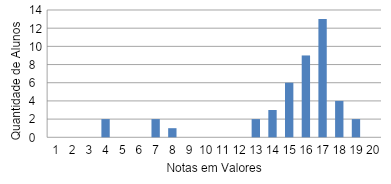
\includegraphics[width=\textwidth]{images/img2.png}
\caption{Resultados da Aplicação da Avaliação Sistemática.}
\label{graf-2}
\source{Produção própria (2022).}
\end{minipage}
\end{figure}

Conforme a Figura \ref{graf-2}, dos resultados da aplicação da avaliação sistemática, percebe-se que:
\newpage
\begin{itemize}
    \item Nos alunos que assistiram ao vídeo até o fim:
    \begin{itemize}
        \item Dos 88,6\% que assistiram ao vídeo até o fim, 71,8\% teve entre 16,0 e 19,0 valores;
        \item Dos 88,6\% que assistiram ao vídeo até o fim, 28,2\% teve entre 13,0 e 15,0 valores.
        \end{itemize}
    \item Nos alunos que assistiram e não terminaram (6,8\%), a nota variou de sete a nove valores.
    \item Nos alunos que não assistiram ao vídeo (4,5\%), a nota variou de zero a cinco valores.
\end{itemize}

Como defende \textcite{deckert2010}, o mais crucial não é assistir, sendo que há uma necessidade de tomar-se nota do que se assistiu e trocar-se ideias sobre o vídeo assistido, de modo a se analisar e concluir sobre o tema em questão.

\subsection{Avaliação dos alunos ao vídeo partilhado}
Em linhas mestras, com o intuito de colher a opinião dos alunos sobre o vídeo publicado na Plataforma do WhatsApp, o Professor de Desenho e Geometria Descritiva aplicou, entre os dias sete e 11 do mês de Março de 2022, uma entrevista semi-estruturada aos alunos da Turma da 11ª C01.

Em relação ao vídeo, o autor solicitou a avaliação aos alunos, via Google Formulário, para atribuição da nota, entre um a dez, tendo em conta o vídeo partilhado na primeira aula sobre o estudo do Ponto, com resultados revelados na Figura \ref{graf-3}, nomeadamente:

\begin{itemize}
    \item Linguagem utilizada no vídeo;
    \item Qualidade do áudio, encenações e cenário;
    \item Qualidade da explicação do conteúdo, e
    \item Realidade do contexto prático do conteúdo abordado.
\end{itemize}

%--- codigo da figura gráfico 3 ---%
\begin{figure}[h!]
\centering
\begin{minipage}{.75\textwidth}
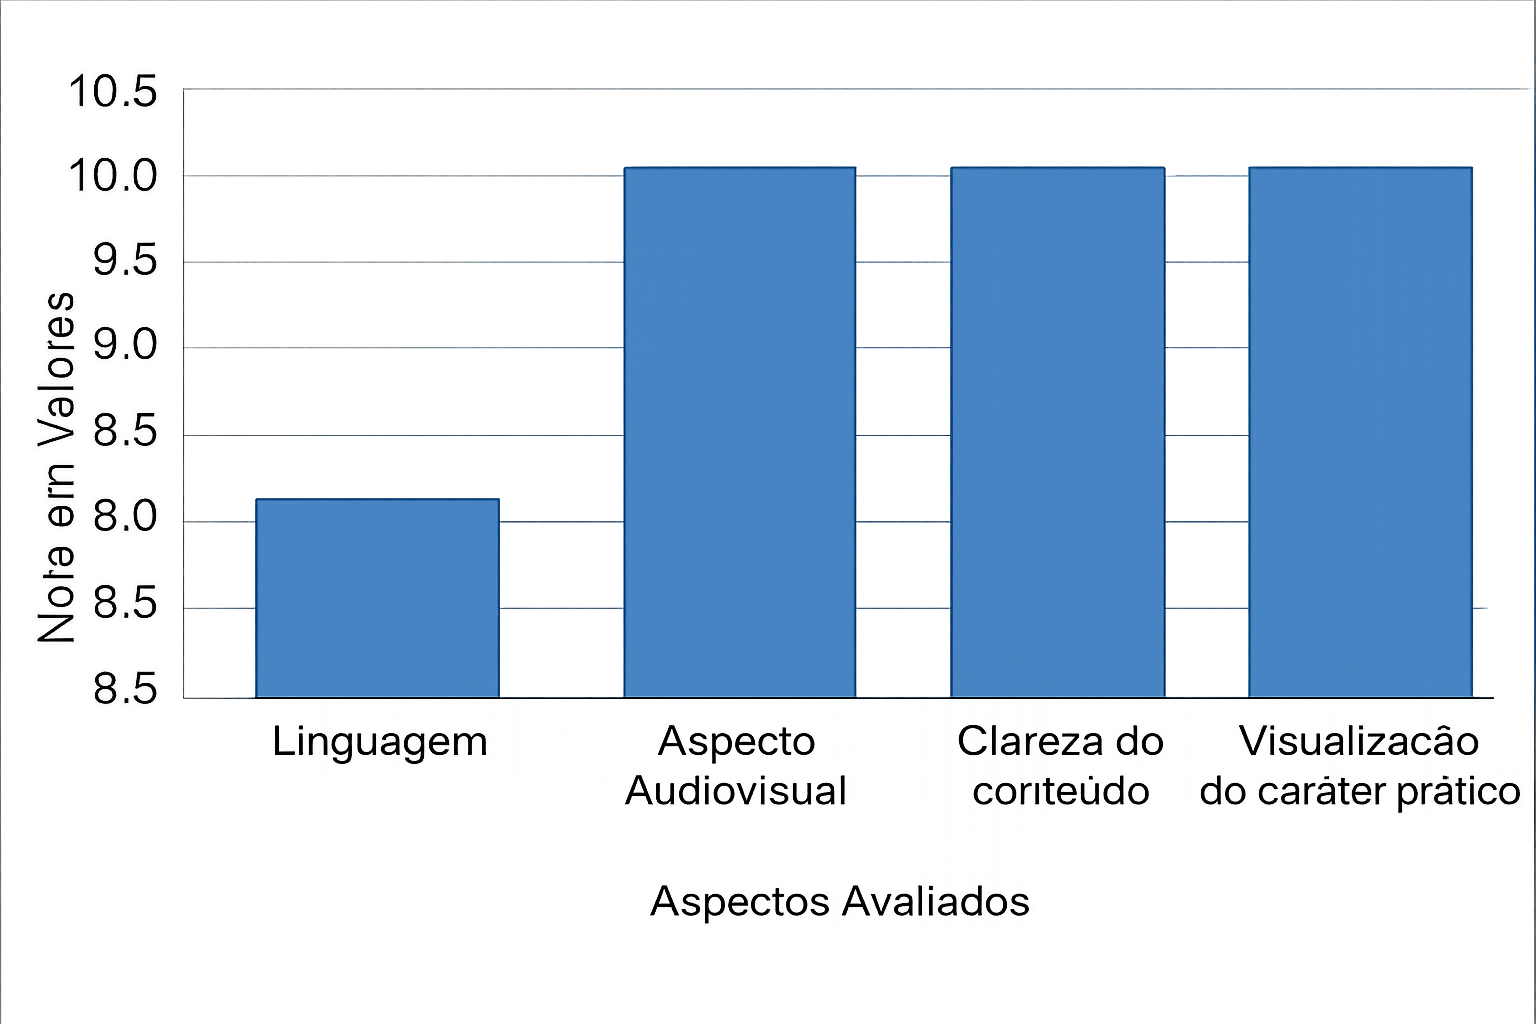
\includegraphics[width=\textwidth]{images/img3.png}
\caption{Resultados da avaliação dos alunos ao vídeo partilhado.}
\label{graf-3}
\source{Produção própria (2022).}
\end{minipage}
\end{figure}

De acordo com a Figura \ref{graf-3}, os alunos avaliaram com nota nove o aspecto da linguagem e atribuíram a nota máxima (10) nas componentes de produção audiovisual, na qualidade do conteúdo partilhado e aplicação do conteúdo na prática, sendo que os alunos se interessaram por novas situações de aprendizagem, como defenderam os pesquisadores \textcite{nicola2016}. Estes autores acrescentam que os alunos se interessam ``quando o recurso utilizado demonstra resultados positivos'' \cite[p. 357]{nicola2016}.

\subsection{Opiniões ao vídeo partilhado}
Por meio da entrevista aos 44 alunos via áudio, foi possível registrar seus comentários sobre o vídeo, entre os quais pode-se destacar:

\begin{quote}
``O tempo do vídeo foi uma das vantagens que minimizou a preguiça'' (Aluno A).

\vspace{0.2\baselineskip}

``Estou sempre a assistir status de WhatsApp, Vídeos no YouTube e Vídeos no TikTok por isso estou habituado e quando o professor partilhou, baixei e assisti com muito gosto'' (Aluno B).

\vspace{0.2\baselineskip}

``Gostei muito, principalmente porque o professor inovou. Com o vídeo nos ajuda a repetirmos a aula sempre que quisermos e se não entendemos alguma coisa é só recuarmos o vídeo'' (Aluno C).
\end{quote}

Esta tendência de respostas é defendida por \textcite{silveira2020}, quando argumentam que os alunos se conectam facilmente aos meios audiovisuais devido a sua normal conexão com a televisão que faz parte do seu quotidiano.

Portanto, estes resultados tiveram suporte na cultura e influência do uso da televisão, pois a experiência e as falas dos alunos revelaram que a televisão, no contexto da Cidade de Chókwè, figura nas três primeiras Tecnologias de Informação e Comunicação, incluindo a rádio e o recente domínio popular da telefonia móvel através de redes sociais.

\section{Considerações finais}\label{sec-cinco}
Portanto, os vídeos representam um bom recurso didático ao estudo de Desenho e Geometria Descritiva, desde que a seleção dos vídeos e a linguagem adotada sejam adequadas ao público-alvo a ser atendido. Durante o artigo, percebeu-se que num total de 44 alunos, 89,6\% assistiram até o fim o vídeo sobre o estudo do ponto, partilhado pelo professor, 6,8\% dos alunos iniciaram com o vídeo e não terminaram, 2,3\% baixaram o vídeo e não assistiram e 2,3\% dos alunos não acederam a plataforma WhatsApp com o vídeo partilhado pelo professor. Nos resultados da aplicação da avaliação sistemática verificou-se a melhoria da qualidade do traço e a exatidão nas respostas.

Outrossim, os alunos avaliaram o vídeo partilhado pelo professor, com nota nove para o aspecto da linguagem e atribuíram a nota máxima (10) a componente audiovisual, a qualidade da explicação no vídeo e aplicação do conteúdo na prática. Dessa forma, os alunos se interessaram por novas situações de aprendizagem e foi uma evidência de que o recurso utilizado demonstra resultados positivos.

Verificou-se que houve uma tendência de respostas que indicaram que os alunos se conectam facilmente aos meios audiovisuais devido a sua normal conexão com a televisão que faz parte do seu quotidiano. Ainda mais, foi bastante notável que há maior interesse em aprender um determinado conteúdo pelo educando.

Assim, como recurso, o vídeo foi considerado motivador no processo do ensino-aprendizagem. Neste sentido, a aplicação do vídeo no ensino ajuda a tornar o ambiente escolar mais interativo e atrativo, criando facilidades de coordenação entre professores e alunos.

Numa outra vertente, importa destacar que uma das constatações é que a maioria dos alunos revela pouco interesse nas aulas tradicionalistas, sendo que o professor pode produzir os vídeos de modo a utilizar como ferramentas que facilitam a aprendizagem de Desenho e Geometria Descritiva.

Se, por um lado, os vídeos quando devidamente produzidos e a sugerirem a resolução de desafios sobre o tema da aula podem favorecer um ambiente inovador na aula, estimulando a participação dos alunos através de questionamentos e seu interesse na aula. Além disso, a tecnologia em Geometria Descritiva pode ser encarada como uma inovação que estimula o processo do ensino e da aprendizagem, a construção de opiniões, críticas e debates no seio dos alunos.

Finalmente, foi notável a eficácia do vídeo no reforço e na motivação significativa na aprendizagem do Ponto. Por isso, propõe-se a produção dos vídeos e sua partilha através das plataformas virtuais mais acessíveis como WhatsApp, Facebook ou Tiktok.

Como futuras pesquisas podem ser realizadas experiências utilizando a metodologia de microlearning, que facilita a construção de conhecimento em alunos da 8ª, 9ª e 10ª Classes, com o foco geral de estimular mais aderência ao Grupo C, que tem registrado pouca aderência devido aos mitos associados nas escolas secundárias em Moçambique.

\phantomsection
\printbibliography\label{sec-bib}
% if the text is not in Portuguese, it might be necessary to use the code below instead to print the correct ABNT abbreviations [s.n.], [s.l.]
%\begin{portuguese}
%\printbibliography[title={Bibliography}]
%\end{portuguese}


\begin{dataavailability}
\txtdataavailability{databody} % options: dataavailable, dataonly, databody, datanotav, nodata
\end{dataavailability}


\end{document}

